\documentclass[12pt]{article}
\usepackage[utf8]{inputenc}

\usepackage{textcomp}
\usepackage[T1]{fontenc}
\usepackage{multirow}
\usepackage{float}
\usepackage[caption = false]{subfig}
\usepackage{longtable}
\usepackage{listings}
\usepackage{mathtools}
\DeclareMathOperator{\tr}{Tr}
\usepackage{commath}
\usepackage{bbold}
\usepackage{xcolor}
\usepackage{physics}
%\usepackage[margin=1.8cm]{geometry}

\usepackage{tikz-cd}
\usepackage{amsmath}
\usepackage{amsfonts}
\usepackage{amssymb}
\usepackage{amsthm}
\usepackage{graphicx}
\usepackage[colorinlistoftodos]{todonotes}
\usepackage[colorlinks=true, allcolors=blue]{hyperref}
\usepackage{siunitx}
\sisetup{separate-uncertainty=true}

\usepackage[sc]{mathpazo}
\linespread{1.05}         % Palladio needs more leading (space between lines)
\usepackage[T1]{fontenc}

\newcommand{\diag}[1]{\text{diag}\qty(#1)}
\newcommand{\const}{\text{const}}
\newcommand{\sign}[1]{\text{sign}\qty(#1)}
\renewcommand{\H}{\mathcal{H}}
\renewcommand{\dim}{\text{dim}}
\newcommand{\C}{\mathbb{C}}
\newcommand{\R}{\mathbb{R}}
\newcommand{\N}{\mathbb{N}}
\newcommand{\Z}{\mathbb{Z}}

\renewcommand{\var}[1]{\text{var} \qty(#1)}
\newcommand{\average}[1]{\langle #1 \rangle}

\newcommand\mybox[1]{%
  \fbox{\begin{minipage}{0.9\textwidth}#1\end{minipage}}}

\usepackage[italian]{babel}
\usepackage{enumitem}

\title{Come fare un azimuth}
\author{}

\begin{document}
\maketitle

\subsection*{Cos'è un azimuth}

Per dare indicazioni su come arrivare da un posto a un altro, possiamo utilizzare un azimuth. 

È necessario dare due informazioni: l'\emph{angolo} rispetto al Nord della direzione dove bisogna andare, e la \emph{distanza} da percorrere in quella direzione. 

\subsection*{Come si misurano gli angoli}

In genere, l'angolo è misurato in \emph{gradi} (sessagesimali), indicati con il simbolo \SI{}{\degree}: l'angolo giro consiste in 360 gradi, o \SI{360}{\degree}. 

\begin{figure}[ht]
\centering
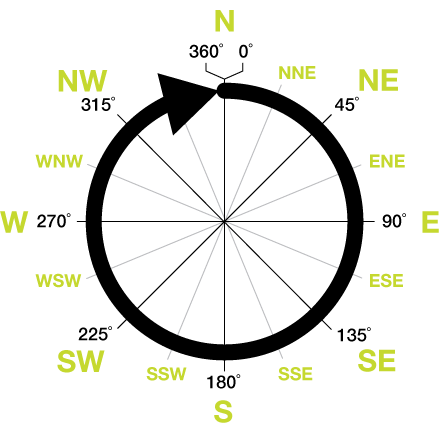
\includegraphics[width=0.7\textwidth]{figures/CompassRoseSimple.png}
\caption{Rosa dei Venti}
\label{fig:rosa-venti}
\end{figure}

Per fare un azimuth gli angoli vanno sempre misurati in senso \emph{orario}. 

Come si può vedere nella figura \ref{fig:rosa-venti}, alla direzione Est corrispondono \SI{90}{\degree}, al Sud \SI{180}{\degree}, all'Ovest \SI{270}{\degree}, mentre al Nord possono corrispondere sia \SI{0}{\degree} che \SI{360}{\degree}: questo significa che un angolo poco a sinistra del Nord misurerà poco meno di \SI{360}{\degree}, mentre un angolo poco a destra del Nord misurerà poco più di \SI{0}{\degree}. Non usiamo valori negativi o maggiori di \SI{360}{\degree}. 

Per avere maggiore chiarezza talvolta aggiungiamo all'angolo l'indicazione N, ad esempio scrivendo ``\SI{30}{\degree}N'', che si legge ``trenta gradi Nord'': questo significa semplicemente che stiamo misurando a partire dalla direzione Nord. 

% La discontinuità in questa rappresentazione è una caratteristica del cerchio visto come varietà differenziabile, \(S^{1}\): non è possibile costruire un atlante con una sola carta che fornisca una rappresentazione \emph{continua} dei punti della varietà su di un aperto di \(\mathbb{R}\), per avere la continuità dovremo usare almeno due carte. 

\subsection*{Come si misurano le distanze}

Le distanze con le quali abbiamo comunemente a che fare si misurano in metri o kilometri. 
Un kilometro corrisponde a mille metri: \(\SI{1}{km} = \SI{1000}{m}\). 

Se non abbiamo a disposizione altro, possiamo misurare una distanza in passi: in genere, un passo è un po' meno di un metro. Per un adulto medio, la lunghezza è di circa \SI{75}{cm}, ovvero tre quarti di metro (\(\SI{1}{m }  = \SI{100}{cm}\)).

Una cosa utile da sapere è esattamente quanto è lungo il nostro passo: basta provare a fare un passo normale, stare fermi e far misurare a qualcun altro quanto sono separati i talloni o le punte dei nostri piedi (attenzione a non misurare dal tallone di un piede alla punta dell'altro! in qual caso avremo misurato il passo più la lunghezza del piede). 

Se sappiamo quanto è lungo il nostro passo, possiamo stimare una lunghezza semplicemente camminando in linea retta e contando i passi. 

Se, invece, abbiamo a disposizione una cartina, possiamo fare una misura più precisa. 

La cartina è una rappresentazione \emph{in scala}, ovvero rimpicciolita, di una certa regione. Ad esempio, le cartine Tabacco che usiamo spesso sono rappresentazioni ridotte di \num{25000} volte della realtà: quindi, un centimetro sulla cartina Tabacco corrisponde a \num{25000} centimetri sul territorio. In metri, avremo: 
%
\begin{align}
\SI{25000}{cm} = \num{25000} \times \qty(\frac{\SI{}{m}}{100}) = \frac{\num{25000}}{100} \SI{}{m} = \SI{250}{m}
\,,
\end{align}
%
quindi 4 centrimetri sulla cartina corrispondono a \(4 \times \SI{250}{m} = \SI{1000}{m} = \SI{1}{km}\). 

La scala della cartina spesso si indica con un simbolo di divisione: ad esempio, la scala della cartina Tabacco si scrive come \(1 : \num{25000}\). 

Quindi, se vogliamo misurare una distanza su una cartina Tabaccco è sufficiente misurarla in centimetri con il righello e poi moltiplicare per 250: così otterremo la distanza in metri. 

\subsection*{Come si calcola un azimuth}

L'azimuth si può misurare sia nel mondo reale che sulla cartina. 

\begin{itemize}[label=$-$]
  \item Per misurare un angolo \textbf{sulla cartina} servono un goniometro e un righello o altro oggetto rettilineo. Centriamo il goniometro sulla posizione dalla quale vogliamo calcolare l'azimuth e allineiamo l'angolo marcato 0 sul goniometro con la direzione Nord della cartina. 
  
  Dopodiché, mettiamo il righello in modo tale che il suo bordo tocchi sia il centro del goniometro, sia il punto il quale azimuth vogliamo calcolare. Allora, il punto dove il righello passa per il goniometro corrisponde all'angolo cercato.
  
  \emph{Attenzione} a leggere l'angolo dall'anello giusto: talvolta in bussole e goniometri ci sono anche altre scale, ad esempio una nella quale l'angolo giro è diviso in 100 gradi (centesimali). La scala che ci interessa è quella che va da 0 a 360 gradi. 

  Per misurare la distanza, possiamo direttamente utilizzare il righello: una volta che abbiamo letto la distanza in centimetri o millimetri sulla cartina, possiamo convertirla in metri o kilometri come spiegato sopra.  
  \item Per misurare un azimuth \textbf{dal vivo} servono una bussola con traguardo e un modo per misurare la distanza. 
  
  Per misurare l'angolo, ci mettiamo nella posizione dalla quale vogliamo misurare l'azimuth e utilizziamo il \emph{traguardo} della bussola: alzando il coperchio della bussola troviamo una fenditura, con al centro un filo. 
  Facendo attenzione a tenere la bussola orizzontale, guardiamo attraverso la fenditura in modo tale da vedere il filo allineato con la direzione desiderata. 

  A questo punto, sul cerchio della bussola possiamo leggere l'azimuth. 

  Per misurare la distanza possiamo usare i passi, come spiegato sopra. 
\end{itemize}

\end{document}